%%%%%%%%%%%%%%%%%%%%%%%%%%%%%%%%%%%%%%%%%
% Simple Sectioned Essay Template
% LaTeX Template
%
% This template has been downloaded from:
% http://www.latextemplates.com
%
% Note:
% The \lipsum[#] commands throughout this template generate dummy text
% to fill the template out. These commands should all be removed when 
% writing essay content.
%
%%%%%%%%%%%%%%%%%%%%%%%%%%%%%%%%%%%%%%%%%

%----------------------------------------------------------------------------------------
%	PACKAGES AND OTHER DOCUMENT CONFIGURATIONS
%----------------------------------------------------------------------------------------

\documentclass[12pt]{article} % Default font size is 12pt, it can be changed here
\usepackage[italian]{babel}
\usepackage[utf8x]{inputenc}
\usepackage[T1]{fontenc}
\usepackage[hmarginratio=1:1,top=32mm,left=20mm,right=20mm,bottom=32mm,columnsep=20pt]{geometry} % Required to change the page size to A4
\geometry{a4paper} % Set the page size to be A4 as opposed to the default US Letter

\usepackage{graphicx} % Required for including pictures

\usepackage{float} % Allows putting an [H] in \begin{figure} to specify the exact location of the figure
\usepackage{wrapfig} % Allows in-line images such as the example fish picture
\usepackage[pdfborder={0 0 0 [0 0]}]{hyperref} % For hyperlinks in the PDF
\usepackage{lipsum} % Used for inserting dummy 'Lorem ipsum' text into the template

\usepackage{color}
\usepackage{lastpage}
\usepackage{enumitem}
\usepackage{fancyhdr} % Headers and footers
\pagestyle{fancy} % All pages have headers and footers
%\fancyhead{} % Blank out the default header
\fancyfoot{} % Blank out the default footer
%\fancyhead[C]{CPNetSolver} % Custom header text
\fancyfoot[C]{\thepage/\pageref{LastPage}} % Custom footer text
\graphicspath{{images/}}

\linespread{1.2} % Line spacing

%\setlength\parindent{0pt} % Uncomment to remove all indentation from paragraphs

\begin{document}

%----------------------------------------------------------------------------------------
%	TITLE PAGE
%----------------------------------------------------------------------------------------

\begin{titlepage}

\newcommand{\HRule}{\rule{\linewidth}{0.5mm}} % Defines a new command for the horizontal lines, change thickness here

\center % Center everything on the page

\textsc{\LARGE Università degli Studi di Padova}\\[1.5cm] % Name of your university/college

\begin{figure}[htbp]
    \centering
      
\includegraphics[scale=0.25]{unipd.png}
\end{figure}

\textsc{\Large Corso di Laurea Magistrale in Informatica}\\[0.5cm] % Major heading such as course name
\textsc{\large Sistemi con Vincoli}\\[0.5cm] % Minor heading such as course title

\HRule \\[0.4cm]
{ \large \bfseries CPNetSolver: applicazione per la risoluzione di CPNet (a)cicliche}\\[0.4cm] % Title of your document
\HRule \\[1.5cm]

%\begin{minipage}{0.4\textwidth}
%\begin{flushleft} \large
%\emph{Author:}\\
%John \textsc{Smith} % Your name
%\end{flushleft}
%\end{minipage}
%~
%\begin{minipage}{0.4\textwidth}
%\begin{flushright} \large
%\emph{Supervisor:} \\
%Dr. James \textsc{Smith} % Supervisor's Name
%\end{flushright}
%\end{minipage}\\[4cm]

\begin{center}
  \emph{Autori:}\\
  Francesco \textsc{Burato}\\
  Simone \textsc{Carriero}\\[2cm]
\end{center}
{\large 12 settembre 2013}\\[3cm] % Date, change the \today to a set date if you want to be precise

%\includegraphics{Logo}\\[1cm] % Include a department/university logo - this will require the graphicx package

\vfill % Fill the rest of the page with whitespace

\end{titlepage}

%----------------------------------------------------------------------------------------
%	TABLE OF CONTENTS
%----------------------------------------------------------------------------------------

\tableofcontents % Include a table of contents

\newpage % Begins the essay on a new page instead of on the same page as the table of contents 

%----------------------------------------------------------------------------------------
%	CONTENT
%----------------------------------------------------------------------------------------

\section{Introduzione}
\begin{frame}{Introduzione}

Cos'è CPNetSolver
\begin{itemize}
  \item risoluzione di CP-Net
  \item visualizzazione grafo dell'ordine degli assegnamenti
  \item accetta anche CP-Net cicliche
\end{itemize}
\end{frame}

\begin{frame}{Introduzione}

Funzionamento:
\begin{itemize}
  \item accettazione CP-Net in input
        %(DIRE:grammatica pross. slide)
  \item conversione da CP-Net a CSP
  \item calcolo e visualizzazione soluzioni ottime
  \item generazione e visualizzazione grafo dell'ordine degli assegnamenti
\end{itemize}

Idea iniziale:
\begin{itemize}
  \item strumento didattico!
  %(DIRE:in ciascun momento si può cambiare la CP-Net
  %corrente e vedere come cambiano le soluzioni e gli ordinamenti)
  
\end{itemize}
\end{frame}

\begin{frame}[fragile]{Introduzione}

Grammatica
\begin{itemize}
\item
\begin{verbatim}
var X dependsOn={}
dom={x,!x}
:x>!x

var Y dependsOn={}
dom={y,!y}
:y>!y

var Z dependsOn={X,Y}
dom={z,!z}
x,y:z>!z
x,!y:!z>z
!x,y:!z>z
!x,!y:!z>z
\end{verbatim}
\end{itemize}
\end{frame}

\newpage
\section{Rappresentazione oggetti}

\subsection{Domini}
Il dominio di una variabile è rappresentato da un \texttt{Set} di \texttt{String} contenente tutti i valori accettati per quella variabile.
L'operazione principale che si può compiere su un dominio è \texttt{contains(elem: String): Boolean} che è usata per verificare se un elemento è contenuto o meno in quel dominio.
\subsection{Ordini}
Gli ordini di una CP-Net, come è noto, sono delle informazioni che
consentono di determinare tra due assegnamenti alle variabili del
problema, nel contesto della semantica dei flip peggiorativi, quale
delle due rappresenti un'assegnamento maggiormente preferito.

Le informazioni irrinunciabili per costruire un ordine sono:
\begin{itemize}
\item Il nome della variabile (e quindi il corrispondente dominio) cui
  l'ordine si riferisce,
\item L'elenco delle eventuali dipendenze,
\item Una mappa che associ ad ogni assegnamento delle variabili di
  dipendenza un ordine totale degli elementi della variabile.
\end{itemize}

La rappresentazione in memoria che è stata scelta per gli ordini è una
struttura dati ad albero. Il motivo di tale scelta risiede nel fatto
che l'utilità dell'ordine è inversamente proporzionale alla quantità
di tempo necessario per indivduare quale è l'ordinamento dei valori
della variabile nel contesto di un certo assegnamento delle variabili
di dipendenza. Date le caratteristiche delle CPNet (a)cicliche è
infatti evidente che se una variabile A dipende dalle variabili B, C e
D, allora la quantità complessiva di ordini totali degli elementi di A
è esattamente pari a $ |dom(B)| \cdot |dom(C)| \cdot |dom(D)| $. La
ricerca di un ordine particolare richiederebbe l'individuazione di una
tupla di elementi di B, C e D all'interno di una struttura dati e la
soluzione che si è adotatta consente di avere un occupazione di
memoria, nell'esempio in esame, di $ O(|dom(A)| \cdot |dom(B)| \cdot
|dom(C)| \cdot |dom(D)|)$ (la minima necessaria per memorizzare un
ordine - $ O(|dom(A)|) $ - per ogni possibile tupla - $ O(|dom(B)|
\cdot |dom(C)| \cdot |dom(D)|)$), e un tempo di ricerca di un ordine
di $O(|dom(A)|+|dom(B)|+|dom(C)|+|dom(D)|)$ (tuttavia migliorabile ad
$O(1)$ come risulterà chiaro dalle sezioni successive).

\subsubsection{Struttura ad albero}
Nella rappresentazione ad albero utilizzata, a ciascun livello di
profondità dalla radice è associata una variabile da cui dipende la
variabile dell'ordine. Nell'esempio presentato nella sezione
precedente, la variabile B sarebbe associata alla profondità 0, la
variabile C alla profondità 1 e la variabile D alla profondità
2. L'ordine in cui una variabile è associata ad una profondità non è
rilevante in termini di prestazioni.

In corrispondenza della profondità associata a ciascuna variabile di
dipendenza, si trovano sempre dei \emph{nodi interni} mentre alla
profondità massima si trovano solo \emph{nodi foglia}. Ad un nodo
interno di profondità \emph{i} è memorizzato un array contenente tutti
i valori che la variabile associata al livello di profondità \emph{i}
può assumere e un puntatore al successivo nodo dell'albero associato a
tale assegnamento. Ad un nodo foglia è associato invece un ordine,
rappresentato come mappa tra stringhe e interi, che interessa la
variabile dell'ordine. Il principio di funzionamento si basa sul fatto
che per arrivare ad un nodo foglia di profondità $n+1$, è necessario
seguire i puntatori di $n$ nodi interni memorizzati assieme a dei
valori assunti dalla variabile associata a ciascun livello di
profondità; l'ordine contenuto in tale nodo foglia è quindi quello
associato al contesto ricostruito dalla radice all'ultimo nodo
interno, assegnando ad ogni variabile di ogni livello di profondità il
valore seguito per costruire il cammino.

Ad esempio, sia $dom(A)=\{a, \overline{a}\}$, $dom(B)=\{b,
\overline{b}\}$, $dom(C)=\{c, \overline{c}\}$, $dom(D)=\{d,
\overline{d}\}$. Per rappresentare gli ordini di A nel caso in cui A
dipenda da B, C e D la struttura a grafo sarà la seguente.

\begin{center}
  \begin{figure}[ht]
    \centering
    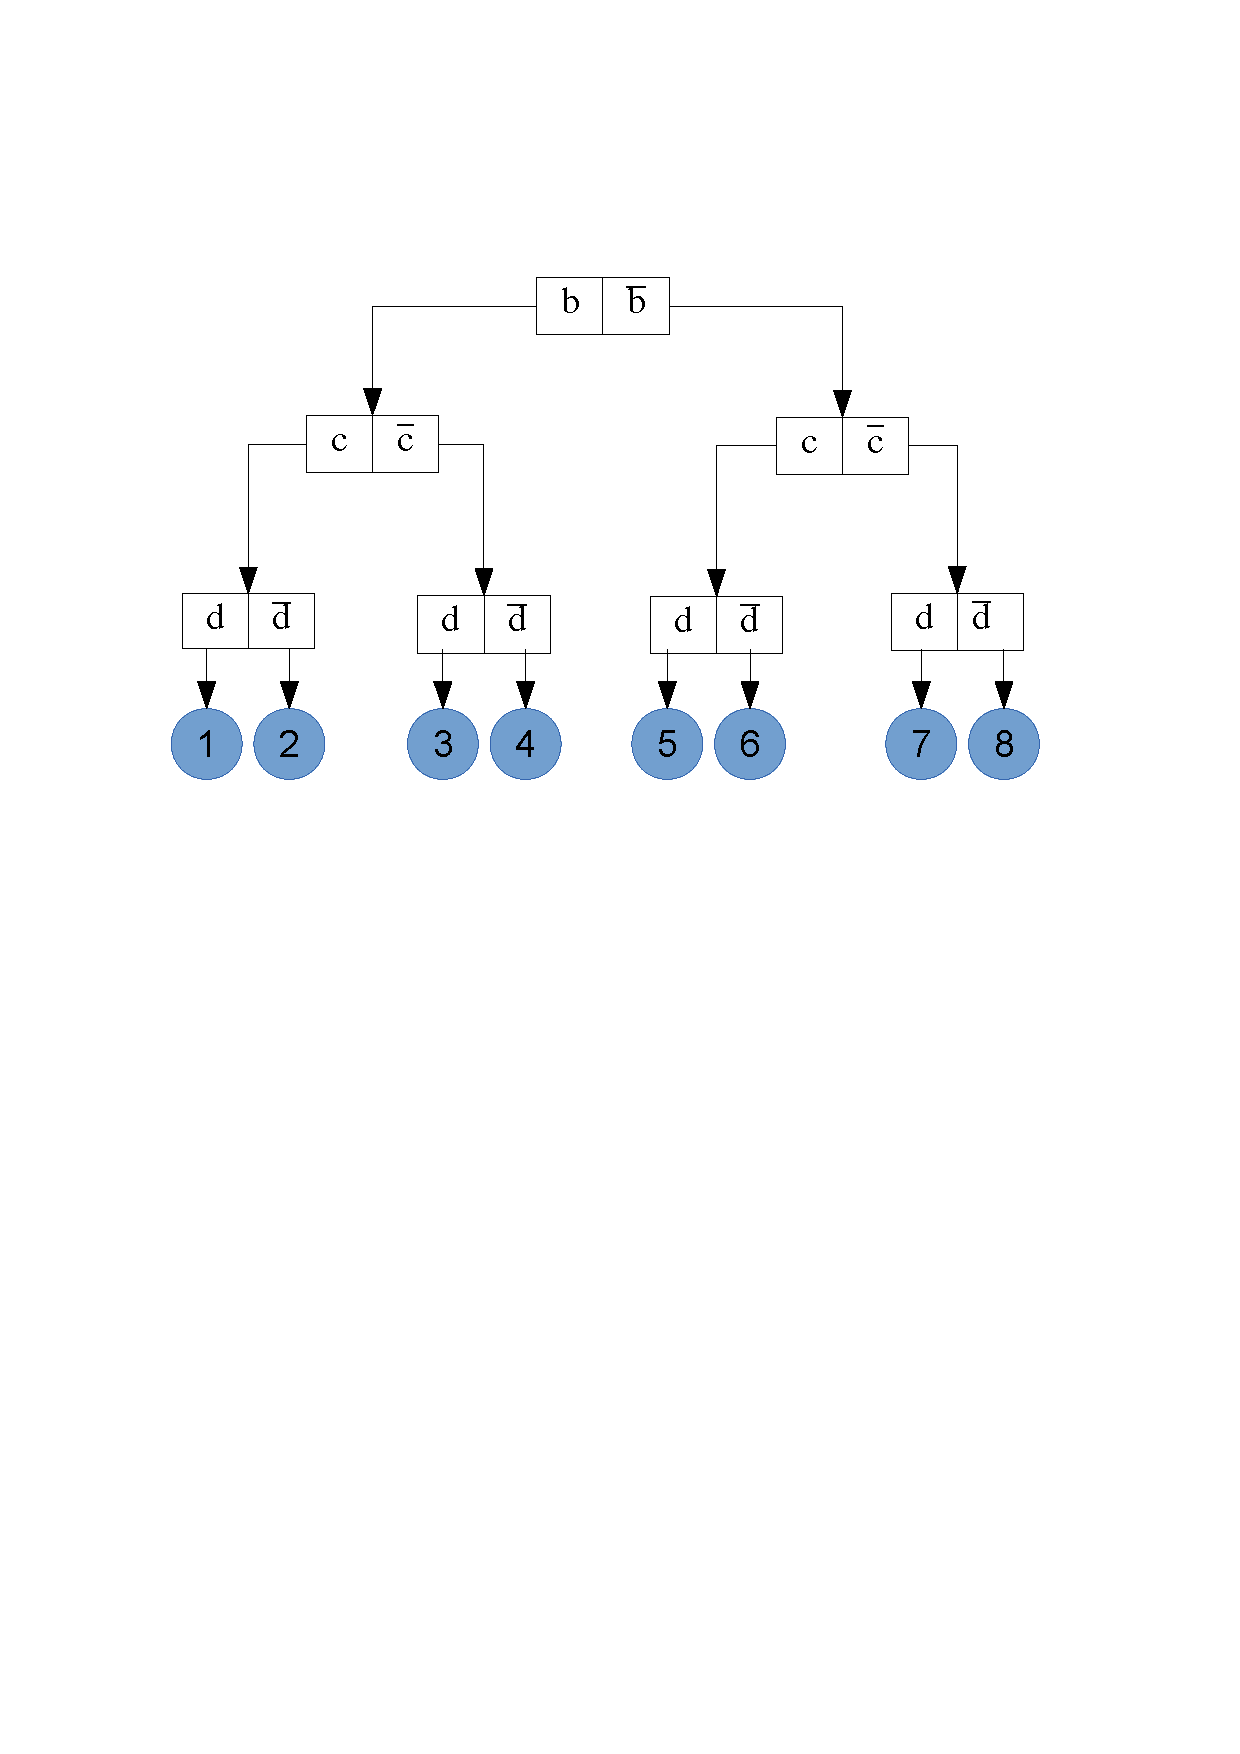
\includegraphics[width=0.5\textwidth]{grafo-ordini}
    \caption{\textit{Rappresentazione a grafo di A, B, C, D}}
  \end{figure}
\end{center}

Nell'esempio si vede chiaramente che per raggiungere ciascuno degli
ordini - ivi rappresentati con dei nodi azzurri numerati - è
necessario costruire un cammino a partire dalla radice alla foglia
relativa all'ordine che equivale ad un assegnamento alle variabili (ad
esempio per raggiungere l'ordine associato ad A identificato con 5 è
necessario assegnare $B=\overline{b}, C=c, D=\overline{d}$).

\subsubsection{Inizializzazione}
Per poter inserire gli ordini è innanzitutto necessario avere a
disposizione la struttura interna dell'albero in cui poi poter
inserire le foglie. Dato che per avere a disposizione una CP-Net
valida è necessario avere tutti gli ordini associati agli assegnamenti
delle variabili di dipendenza, è evidente che sia possibile
inizializzare dapprincipio l'intera struttura interna nel momento in
cui si costruisce l'ordine. Tale struttura infatti dipende unicamente
dalle variabili di dipendenza e dai loro elementi e non è necessaria
alcuna informazione sugli ordini alle foglie per poterla costruire.

All'interno del progetto questa inizializzazione viene effettuata alla
costruzione degli oggetti ordini e la complessità della costruzione è
pari a $O(|dom(V_1)| \cdot \dots \cdot |dom(V_n)|)$ ove $ V_1, \dots,
V_n $ sono tutte le variabili di dipendenza dell'ordine.

\subsubsection{Complessità}
Vista la rappresentazione è quindi evidente che la complessità della
ricerca di un assegnamento $ V_1=v_1, \dots, V_n=v_n $ dipenda da:

\begin{itemize}
\item numero di variabili di dipendenza (n) che comunque si può
  assumere come costante in quanto una volta costruito l'ordine tale
  parametro non cambia mai,
\item ricerca del valore $v_i$ all'interno del nodo interno
  \textit{i-esimo}
\end{itemize}

Dovrebbe risultare quindi evidente che la rappresentazione dei valori
assunti da ogni variabile nei nodi interni determina la complessità
della ricerca. Detta $W$ la variabile a dominio di cardinalità massima
allora
\begin{itemize}
\item se i dati sono memorizzati come array non ordinato allora la
  complessità della ricerca sarà pari a $O(n \cdot
  |dom(W)|)=O(|dom(W)|)$.
\item se i dati sono memorizzati in una struttura dati ordinata allora
  la complessità della ricerca sarà pari a $O(n \cdot
  log|dom(W)|)=O(log|dom(W)|)$.
\item se i dati sono memorizzati in una tabella hash (facile da
  costruire dato che si sa fin dal principio quanti elementi inserire)
  allora la complessità della ricerca sarà pari a $O(n \cdot
  1)=O(n)=O(1)$.
\end{itemize}

\subsubsection{Comparatori}
\label{sect:comparatori}
I Comparatori sono oggetti associati ad un ordine che sono
utilizzabili per costruire la semantica dei flip peggiorativi. L'idea
è che dato un ordine si ha a disposizione l'albero associato a tale
ordine e quindi è facile riuscire a determinare quale è il migliore
tra due assegnamenti che differiscono per un solo valore associato
alla medesima variabile.

Dati gli assegnamenti $X=(V_1=v_1, \dots, V_{i-1}=v_{i-1}, V_i=x,
V_{i+1}=v_{i+1}, \dots, V_m=v_m)$ e $Y=(V_1=v_1, \dots,
V_{i-1}=v_{i-1}, V_i=y, V_{i+1}=v_{i+1}, \dots, V_m=v_m)$\footnote{$m$
  è usato per indicare il numero di variabili del problema} un
comparatore di un ordine associato alla variabile $V_i$ procede come
segue:
\begin{enumerate}
\item Accetta sequenzialmente tutti gli assegnamenti $V_1=v_1, \cdots,
  V_{i-1}=v_{i-1}, V_{i+1}=v_{i+1}, \dots, V_m=v_m)$.
\item Non appena tutte le variabili da cui dipende $V_i$ sono state
  fornite, il comparatore scandisce l'albero dell'ordine di $V_i$ fino
  trovare l'ordine associato all'assegnamento.
\item Trovato l'ordine associato, il comparatore può rispondere al
  confronto tra $x$ e $y$ perché dispone di tutte le informazioni: è
  sufficiente confrontare i valori associati alla mappa dell'ordine a
  $x$ e $y$ per sapere quale dei due è migliore dell'altro.
\end{enumerate}
\subsection{Vincoli}
I vincoli sono rappresentati dalla classe \texttt{Constraint}, caratterizzata dai due seguenti campi dati:
\begin{itemize}
\item \texttt{vars: Array[String]} che rappresenta una lista ordinata di variabili,
\item \texttt{accepted: Buffer[Array[String]]} che rappresenta la lista di tutte le
istanziazioni accettate per quelle variabili.
\end{itemize}

%$O(|dom(V_1)| \cdot \dots \cdot |dom(V_n)|)$ ove $ V_1, \dots, V_n $

Ad esempio, date tre variabili $X,\ Y$ e $Z$ tali che $dom(X)=\{0,1\},\ dom(Y)=\{0,1\}$ e $dom(Z)=\{0,1\}$, l'oggetto di tipo \texttt{Constraint} che
rappresenta il vincolo $X+Y=Z$ avrà
\begin{itemize}
  \item \texttt{vars = [X, Y, Z]} e 
  \item \texttt{accepted = [ [0, 0, 0], [1, 0, 1], [0, 1, 1] ]}.
\end{itemize}


\newpage
\section{Algoritmi}

\subsection{Trasformazione da CP-Net a CSP}
Come accennato in precedenza, la ragione per cui si ha la necessità di
trasformare la CP-Net in un CSP è che l'applicazione permette la risoluzione di
CP-Net cicliche, e per la risoluzione di questo tipo di CP-Net è necessario
effettuare tale trasformazione.

Data una CP-Net è sempre possibile costruire un CSP classico con lo stesso
insieme di soluzioni ottime nel seguento modo: per ogni ordine $X_1=x_1, ...,
X_n=x_n: Y=y_1 > Y=y_2 > ... > Y=y_k$ costruiamo il vincolo $X_1=x_1, ..., X_n=x_n
=> Y=y_1$.

Vista la rappresentazione adottata per gli ordini, questo corrisponde a creare, per
ciascuna variabile $v$, un vincolo per ogni foglia dell'albero degli ordini di $v$.
Infatti, considerato che per ogni foglia si conosce l'istanziazione delle variabili
$X_1=x_1, ..., X_n=x_n$ che è rappresentata da tutti i nodi tra la radice e la
foglia, e il relativo ordine $Y=y_1 > Y=y_2 > ... > Y=y_k$
è possibile costruire il vincolo $X_1=x_1, ..., X_n=x_n => Y=y_1$.

\subsection{Ricerca delle soluzioni}
La ricerca delle soluzioni della CP-Net è fatta attraverso un
algoritmo di tipo Backtracking+Forward Checking modificato per trovare
tutte le soluzioni ottime e non solo una soluzione.

L'algoritmo seguito per risolvere un problema a $m$ variabili è quindi
il seguente:
\begin{enumerate}
\item \textbf{Inizializzazione:} Si raccolgano tutti i domini di tutte
  le variabili del problema e tutti i vincoli ottenuti dalla
  conversione della CP-Net in CSP. Ciò consente di ottenere tutte le
  tuple ammesse dagli assegnamenti delle variabili in un ordine.
\item \textbf{Partenza:} Si esegua la ricerca in profondità partendo
  dal livello 0 avendo come vettore di supporto un vettore vuoto.
\item \textbf{Ricerca in profondità di livello i-esimo e vettore di
    supporto $w$:} Se $i=m$ allora $w$ contiene una soluzione alla
  CP-Net che viene segnalata, altrimenti se il dominio i-esimo è vuoto
  allora vuol dire che l'assegnamento precedente ha causato un
  inconsistenza e la ricerca a questo punto termina, altrimenti per
  ogni valore $v$ del dominio i-esimo:
  \begin{enumerate}
  \item Si riducano i vincoli attuali rispetto a $v$ ovvero si
    ottengono tutte le tuple che ammettono la variabile i-esima
    associata al valore $v$.
  \item Si intersechino i domini correnti con le proiezioni dei
    vincoli ovvero si ottengano tutti e soli i valori ammessi dai
    vincoli per ciascuna variabile avendo ridotto i vincoli 
    con l'$i$-esima variabile assegnata a $v$
  \item Si assegni $w[i]=v$.
  \item Si esegua la ricerca in profondità di livello i+1 con il nuovo
    w come vettore di supporto.
  \end{enumerate}
\end{enumerate}
\subsection{Calcolo diagramma di ordine per gli assegnamenti}
La realizzazione del diagramma di rappresentazione dell'ordine degli assegnamenti necessita innanzitutto di una libreria in grado di gestire e
rappresentare grafi all'interno di un'interfaccia grafica. La scelta è
quindi ricaduta sul ``Java Universal Network/Graph
Framework''\footnote{\url{http://jung.sourceforge.net/}}, una libreria
open source che possiede tutte le caratteristiche necessarie al
progetto.

Una volta che i grafi possono essere rappresentati è necessario
indivduare un modo efficiente per riuscire a calcolare l'ordine degli assegnamenti utilizzando la semantica dei flip peggiorativi. A questo
scopo è stato realizzato un algortimo che è in grado di calcolare in
tempo ammortizzato $O(e + v)$ l'intero diagramma degli ordini, dove
$e$ è il numero di archi del grafo e $v$ il numero di vertici.

\subsubsection{Contatore variabile}
L'astrazione che consente di raggiungere un alta efficienza è quella
del \textit{contatore variabile}. Se un contatore binario è un
contatore in cui tutte gli elementi del contatore lavorano in modulo
2\footnote{Si veda Cormen, Leiserson, Rivest e Stein ``Introduzione
  agli algortimi e Strutture Dati'' - McGraw Hill}, definiamo un
contatore variabile un contatore in cui a ciascun elemento è associato
un diverso insieme quoziente (non solo 2).

Per fare un esempio, in un contatore variabile a 3 elementi i cui
insiemi quozienti siano quelli modulo 5, 7 e 3 una possibile
configurazione degli elementi sarebbe (4,4,2). Un incremento
determinerebbe nel contatore il cambiamento della configurazione a
(4,5,0) in quanto l'aggiunta di 1 all'elemento meno significativo
causa un riporto che deve andare a trasferirsi all'elemento
successivo.

L'utilizzo del contatore variabile all'interno del calcolo dell'ordine
degli assegnamenti consiste nell'impiego di un contatore per riuscire
ad individuare senza ripetizioni tutti i flip peggiorativi di una
configurazione. Per fare ciò si stabilisce un ordine arbitrario a
tutti i valori dei domini di ciascuna variabile e ad ogni elemento del
contatore si associa una variabile ovvero un'insieme quoziente modulo
la cardinalità del dominio di tale variabile. Per evitare le
ripetizioni è sufficiente considerare una configurazione $i$ di un
contatore e calcolare tutte e sole le configurazioni che si ottengono
da $i$ modificando un solo elemento del contatore e che siano
\textit{strettamente maggiori di $i$}.

Ad esempio, considerando il contatore introdotto in precedenza, data
la configurazione $i$=(3,1,0), allora la configurazioni strettamente
maggiori diverse per al più un elemento sono: (3,1,1), (3,1,2),
(3,2,0), (3,3,0), (3,4,0), (3,5,0), (3,6,0), (4,1,0).

Stabilito l'ordine degli elementi per i domini di ogni variabile, dato
un contatore è immediato risalire a quale sia l'assegnamento delle
variabili che è rappresentata dal contatore. Pertanto data una
configurazione di contatore $i$ e le configurazioni strettamente
maggiori di $i$ ottenute con il procedimento precedentemente
descritto, si ottengono un assegnamento di variabili e tutti gli
assegnamenti a distanza 1. Usando i compartori descritti alla sezione
\ref{sect:comparatori} è immediato calcolare quale sia la relazione
esistente di preferenza tra gli assegnamenti.

L'algoritmo per il calcolo degli ordini degli assegnamenti è quindi il
seguente:
\begin{enumerate}
\item \textbf{Inizializzazione:} Si stabilisca un ordine per i valori
  di ciascuna variabile, si estraggano i comparatori dagli ordini di
  ogni variabile, si inizializzi un contatore variabile $c$ ad
  elementi pari alla cardinalità delle variabili, si inizializzi un
  grafo orientato $G$.
\item \textbf{Ciclo di calcolo:} Fino a che $c$ non è arrivato alla
  configurazione massima:
  \begin{enumerate}
  \item Si calcoli l'insieme delle configurazioni strettamente
    maggiori di $c$ distanti 1.
  \item Per ogni configurazione ottenuta al punto (a) si usi il
    comparatore associato all'unica variabile modificata per
    determinare quale delle configurazioni sia preferita e si segnali
    in $G$ la preferenza.
  \item Si incrementi $c$.
  \end{enumerate}
\end{enumerate}

\subsubsection{Complessità}
La complessità dell'algoritmo precedentemente descritto, ipotizzando
che si utilizzi la rappresentazione dei nodi interni degli ordini a
tabella hash, è esattamente pari a $O(e + v)$ in quanto:
\begin{itemize}
\item Tutti i passi di inizializzazione sono costanti e svolti in
  tempo $O(1)$.
\item Il numero di iterazioni del ciclo di calcolo è esattamente
  $O(v)$.
\item Il numero totale di configurazioni strettamente maggiori di $c$
  e distanti 1 nella totalità dell'esecuzione è $O(e)$ e il loro
  calcolo è a tempo costante, quindi il costo totale del passo (a) in
  tutta l'esecuzione è $O(e)$.
\item Con la tabella hash il costo per trovare l'ordine interessato è
  $O(1)$ quindi il costo complessivo del passo (b) in tutta
  l'esecuzione è $O(e)$ in quanto il confronto tra due valori trovato
  l'ordine è svolto in tempo costante.
\item L'incremento del contatore $c$ è realizzabile in tempo
  ammortizzato costante quindi il costo complessivo del passo (c) per l'intera
  esecuzione è $O(v)$.
\end{itemize}

Complessivamente quindi si ha $O(1) + O(e) + O(v)= O(e+v)$.

\newpage
\section{Conclusioni}
CPNetSolver rappresenta un utile strumento per riuscire a risolvere e
visualizzare concretamente una CP-Net, sia essa ciclica o aciclica. Un
ovvio campo di applicazione per tale programma è evidentemente quello
didattico, in quanto la possibilità di modificare con una semplice
grammatica la definizione di una CP-Net e vedere immediatamente quali
sono le conseguenze sul grafo degli ordini degli assegnamenti e sulle
soluzioni, è uno strumento semplice ma estremamente utile per capire
concetti come la semantica dei flip peggiorativi e la necessità degli
ordini completi.

Nonostante si tratti di un'applicazione didattica è stata prestata
molta attenzione ai problemi computazionali e di rappresentazione
degli oggetti del dominio. Inoltre l'impiego di Scala e di uno stile
di programmazione funzionale potrebbe consentire, come ottimizzazione
futura, la possibile parallelizzazione degli algoritmi di calcolo
delle soluzioni ottime e di rappresentazione del grafo degli ordini
degli assegnamenti.


%----------------------------------------------------------------------------------------
%	BIBLIOGRAPHY
%----------------------------------------------------------------------------------------

%\begin{thebibliography}{99} % Bibliography - this is intentionally simple in this template
%
%\bibitem[Figueredo and Wolf, 2009]{Figueredo:2009dg}
%Figueredo, A.~J. and Wolf, P. S.~A. (2009).
%\newblock Assortative pairing and life history strategy - a cross-cultural
%  study.
%\newblock {\em Human Nature}, 20:317--330.
% 
%\end{thebibliography}

%----------------------------------------------------------------------------------------

\end{document}